% !TeX root = ../Ideal-Fluid Flow.tex
\chapter{Introduction}
\section{Ideal-Fluid}
\begin{definition}\mbox{}\\
\[
\textrm{Ideal-fluid}
\left\{
\begin{aligned}
&\textrm{Inviscid }(\mu = 0)\\
&\textrm{Incompressible flow }(\rho=\textrm{constant})
\end{aligned}
\textrm{fluid}
\right.
\]
The flow field generated by such flow $\Longrightarrow$ \emph{Ideal flow}
\end{definition}
\begin{note}\mbox{}\\
More commonly, ideal flow deals with flows which are \emph{inviscid} $(\mu=0)$, \emph{incompressible} $(\rho=\textrm{constant})$, and also \emph{irrotational} $(\nabla\times\mathbf{u}=\mathbf{0})$. Such flows are called \emph{Potential Flows}.
\end{note}
\begin{itemize}
\item Justifications:\\
For real fluids, more and less, $\mu\neq 0$, $\rho\neq$constant.
\begin{enumerate}[label = <\roman*>]
\item Cases when flows can be treated as \emph{inviscid}. Air and water have negligible viscosity. $(\nu = \mu/\rho\sim\mathcal{O}(10^{-5}\sim 10^{-6})\textrm{m\textsuperscript{2}/s})$\label{1-1-i}
\begin{enumerate}[label = \protect\circled{\arabic*}]
\item near a solid body (e.g. boundary layer)
\begin{figure}[H]
\centering
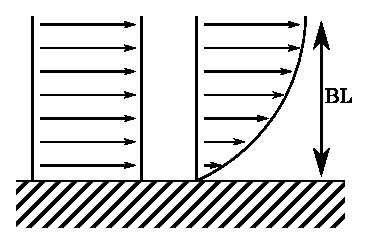
\includegraphics[scale=1.0]{figure/chapter1/1-1-1.eps}
%\caption{Scheme of blowing/suction flow}
%\label{Scheme of blowing/suction flow}
\end{figure}
\item wake
\begin{figure}[H]
\centering
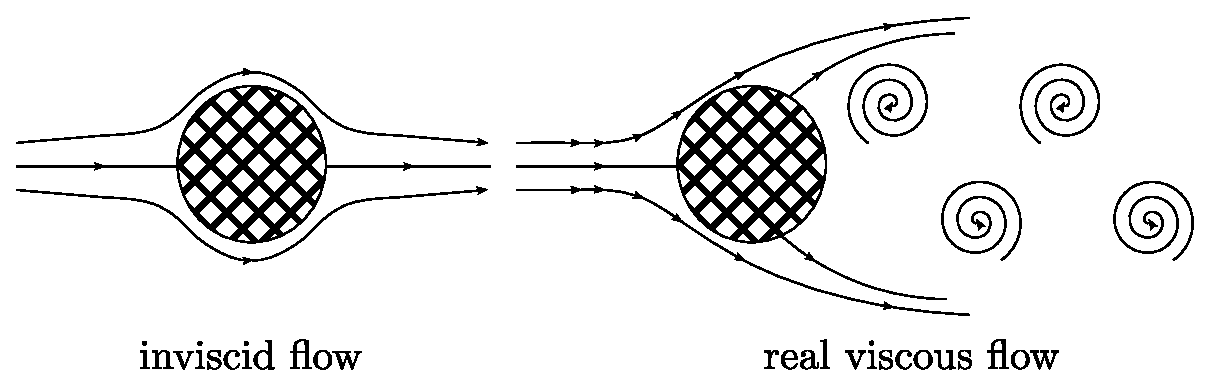
\includegraphics[scale=0.7]{figure/chapter1/1-1-2.eps}
%\caption{Scheme of blowing/suction flow}
%\label{Scheme of blowing/suction flow}
\end{figure}
\item fluid-fluid interface, shock...
\end{enumerate}
In general, viscosity effect can be neglected if $Re = UL/\nu\ll 1$
\item Cases when flows can be treated as \emph{incompressible}.\label{1-1-ii}
\begin{enumerate}[label = (\alph*)]
\item Almost in all cases, the \emph{liquid} can be taken as \emph{incompressible}.
\item For \emph{gases}, we can neglect their compressibility if the variation in density $\Delta p/\rho$ in the flow is $<5\%$.
\begin{enumerate}[label = \protect\circled{\arabic*}]
\item in the case where variation in density is largely due to \emph{pressure change} from Bernoulli's equation.\label{1.1-1}
\[
\frac{d(v^2/2)}{ds} = -\frac{1}{\rho}\frac{dp}{ds}
\]
\begin{equation}
\Longrightarrow\frac{\Delta p}{\rho}\sim\frac{(\Delta v)^2}{2}\sim\frac{U_\infty^2}{2}
\label{eq: 1-1}
\end{equation}
The sound speed ``$a$'' is defined:
\begin{align*}
a = \sqrt{\left.\frac{\partial p}{\partial \rho}\right|_s} = \sqrt{\gamma RT},&& \gamma = \frac{c_p}{c_v}
\end{align*}
\begin{align*}
\therefore a^2 = \gamma RT = \gamma\frac{p}{\rho}, && \boxed{M_\infty = \frac{U_\infty}{a}}\textrm{ (Mach number)}
\end{align*}
\begin{equation}
\Longrightarrow \frac{U_\infty^2}{p/\rho} = \gamma M_\infty^2
\label{eq: 1-2}
\end{equation}
substitute \eqref{eq: 1-2} into \eqref{eq: 1-1}
\begin{equation}
\Longrightarrow \frac{\Delta p}{p}\sim \frac{\gamma}{2}M_\infty^2
\label{eq: 1-3}
\end{equation}
use $p = \rho RT$, take $T\approx$constant,
\begin{equation}
\Longrightarrow\frac{\Delta p}{p}\sim\frac{\Delta\rho}{rho}\Longrightarrow\boxed{\frac{\Delta\rho}{\rho}\sim\frac{\gamma}{2}M_\infty^2}
\label{eq: 1-4}
\end{equation}
For most gases, $\gamma\approx 1$, hence $\Delta\rho/\rho <5\%$ if $\underline{M_\infty <0.3}$.
\item in the case where variation in density is largely due to \emph{temperature change}\label{1.1-2}\\
Assume \emph{adiabatic process}
\begin{align*}
dh = c_pdT, && h + \frac{v^2}{2} = \textrm{constant}
\end{align*}
\begin{equation}
\Longrightarrow\Delta T = \frac{\left(\Delta v\right)^2}{2c_p}\Longrightarrow T_\infty = \frac{U_\infty^2}{2c_p}
\label{eq: 1-5}
\end{equation}
also
\begin{align*}
a^2 = \gamma R T_\infty, && c_p = \frac{\gamma R}{\gamma - 1}
\end{align*}
hence 
\begin{equation}
\eqref{eq: 1-5}\Longrightarrow \frac{\Delta T}{T_\infty} = \frac{\gamma -1}{2}M_\infty^2
\label{eq: 1-6}
\end{equation}
For reversible, adiabatic process,
\begin{align*}
p\rho^{-\gamma} = c && \text{ or }pv^\gamma = c && \text{ or }T\rho^{1-\gamma} = c
\end{align*}
\[
\therefore\frac{\Delta T}{T_\infty}\sim\left(\gamma-1\right)\frac{\Delta\rho}{\rho_\infty}
\]
hence
\begin{equation}
\eqref{eq: 1-6}\Longrightarrow
\boxed{
\frac{\Delta\rho}{\rho_\infty}\sim\frac{M_\infty^2}{2}
}
\label{eq: 1-7}
\end{equation}
\begin{align*}
\frac{\Delta\rho}{\rho_\infty}< 5\% \text{ if }\boxed{M_\infty< 0.3}
\end{align*}
\end{enumerate}
\end{enumerate}
\end{enumerate}
$
\left.
\begin{aligned}
&\ref{1.1-1} \\
&\ref{1.1-2}
\end{aligned}
\right\}
\Longrightarrow$
In general, the flow can be treated as incompressible if $M_\infty <0.3\%$.

Combine \ref{1-1-i} and \ref{1-1-ii}, the flow can be treated as an Ideal flow if 
$\left\{
\begin{aligned}
&Re \gg 1\\
&M < 0
\end{aligned}\right.$\\
except region
$\left\{
\begin{aligned}
&\text{Boundary layer} (BL)\\
&\text{Wake} \\
&\text{shock}
\end{aligned}\right.
$
\item Applications: 
\begin{enumerate}[label = \protect\circled{\arabic*}]
\item Hydraulic (e.g. Bernoulli's equation) \\
\item Surface waves
\item Aerodynamics (e.g. Thin-airfoil Theory)
\end{enumerate}
\end{itemize}
